\section{Analysis}
\label{sect:signal_types}
The most common transmissions sought in SETI searches are narrow-band ($\sim$Hz) radio signals. Ubiquitous in early terrestrial communication systems, such signals can be produced with relatively low energy and traverse the interstellar medium easily. They can be readily distinguished from natural astrophysical sources. These signals could either be transmitted intentionally or arise as leakage from extra-solar technologies. The apparent frequency of a distant narrow-band transmitter is expected to exhibit Doppler drift due to the relative motion between the transmitter and receiver. 
The Breakthrough Listen group has developed an efficient narrow-band search software package which includes a search for such drifting signals, named \verb|turboSETI|~\citep{Enriquez:2017} which we use for the analysis of our LOFAR survey data. However, before we can compare narrowband signal hits detected using this tool, it was necessary to compare them in the Barycentric reference frame. 

\begin{figure}
    \centering
    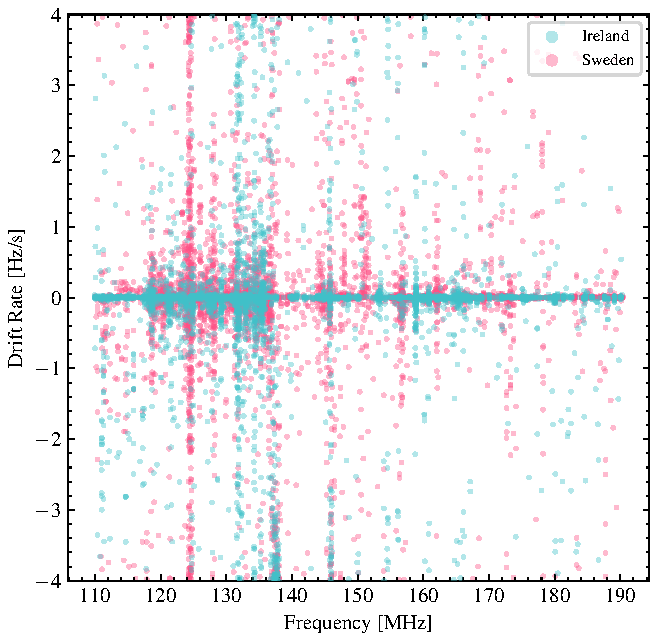
\includegraphics[width = 0.45\textwidth]{SETI/figures/narrowband/DR_scatter_plot.pdf}
    \caption{A scatter plot of the drift rate values against detected frequency. The Irish station is shown in pink and the Swedish station is shown in blue.}
    \label{fig:scatter_DR}
\end{figure}

\subsection{Barycentric correction}
The movement of the Earth around its axis and the Sun introduces a Doppler effect that causes radio signals' frequency and arrival time to shift, as 
\begin{equation}
f_{obs} = f_{em} \left( 1 - v_{rel} \right).
\label{eq:doppler}
\end{equation}
Here, $f_{obs}$ is the observed frequency, $f_{em}$ is the emitted frequency (or barycentric frequency), and $v_{rel}$ is the velocity of the source relative to the observer, normalized by the speed of light. The Doppler effect only depends on the velocity of the source relative to the observer, and for a source moving towards the observer, we can consider $-v_{rel}$, while for a source moving away from the observer, we consider $+v_{rel}$. The relative velocity between the observer and the source will differ for different observing epochs, the location of the source in the sky, and the geographical location of the telescope. For instance, the target TIC\,27677846 was observed on UT 2021 July 15, from both the LOFAR stations simultaneously. The expected relative velocity ($v_{rel}$) towards the source was $-7.669\times10^{-5}$ and $-7.496\times10^{-5}$, causing a relative shift ($f_{em}-f_{obs}$) of +11.504\,kHz and +11.246\,kHz for a hypothetical ETI signal transmitted at a constant frequency of 150\,MHz observed at the Sweden and Ireland stations, respectively. These are significant shifts that are distinct at the two stations, and they need to be corrected to compare the same signal observed at the two stations. 

Typically, barycentric corrections are introduced by adjusting the local oscillator during observations. However, in our study, we record beamformed baseband voltages during observations and produce three different data products with varying temporal and spectral resolutions during post-processing \citep{2019_Lebofsky}. We are interested in searching for a wide variety of signals, including narrowband signals, broadband transient signals, and wide-band pulsating signals. Introducing local oscillator shifts during observations can impact our other signal searches. Therefore, we correct for barycentric drift after the channelization and detection of the baseband voltages for narrowband signal searches using software which we have developed\footnote{\url{https://github.com/gajjarv/BaryCentricCorrection}}. Details of this correction and code \citep{Vishal_Bary} are fully discussed in Appendix~\ref{appen:barycenter}. For comparison both topocentric and barycentric data are analysed for a small sub-set of the targets and the results are shown in Table \ref{tab:barycenter_vs_topocenter}. 


\begin{table}[ht]
  \centering
  \begin{tabular}{lccc|ccc}
  \hline
  \textbf{TIC ID} & \multicolumn{3}{c|}{\textbf{Topocentric Results}} & \multicolumn{3}{c}{\textbf{Barycentric Results}} \\
   & LOFAR-SE Hits & I-LOFAR Hits & Mutual Hits & LOFAR-SE Hits & I-LOFAR Hits & Mutual Hits \\
  \hline
  121966220 & 387 & 178 & 18 & 376 & 171 & 0 \\
  249862365 & 340 & 193 & 22 & 330 & 196 & 0 \\
  250724252 & 276 & 190 & 21 & 265 & 262 & 0 \\
  27677846  & 313 & 159 & 20 & 294 & 151 & 0 \\
  470315428 & 384 & 175 & 17 & 356 & 224 & 0 \\
  \hline
  \end{tabular}
  \caption{Comparison of the number of narrow-band signals detected for a subset of \textit{TESS} objects in both the topocentric and barycentric reference frame. \texttt{turboSETI} searches were completed using identical parameters in each reference frame. A small number of mutual hits were found in the topocentric frame, but these were filtered out entirely in the barycentric case.}
  \label{tab:narrowband_hit_bary_non_bary_compare}
  \end{table}
  

\subsection{Searching for Narrowband Signals}
Using \verb|turboSETI| with the parameters outlined in Table \ref{tab:data_details}, a Doppler drift search was carried out on the observed candidates listed in \Cref{tab:TESS_results} and \ref{tab:Gaia_results} at both stations. This resulted in the list of `hits' collected in Tables \ref{tab:TESS_results} and \ref{tab:Gaia_results}, where hits are defined as a narrow-band signal detected above the given threshold, S/N = 10. The distribution of narrow-band signals detected at both stations is shown in \Cref{fig:histogram_hits_comparison}. A large percentage of hits are seen at both sites in the 120 - 140 MHz range. This falls within the range of expected RFI leakage seen from neighboring airports\footnote{Shannon \& Goteborg Landvetter}. \\

Using a drift-rate search of $\pm 4 \ \text{Hz/s}$ for this study covers a fraction of the possible drift rates of transmitters from exotic objects that can be detected as outlined by \cite{Sheikh_2019}. \cite{LiNarrowBand} shows that 4~Hs/s is comprehensive in relative to the expected distribution of exoplanet drift rates. The omission of a search in this parameter space is due to its computationally intense nature of searching for narrow-band signals across a sizeable drift-rate range. However, in doing this, the parameter space searched for ETI signal has been drastically reduced. Continual development of search algorithms like \verb|turboSETI| is progressing to make larger drift-rates searches a more computationally feasible. \\ 

Upon first inspection of \Cref{fig:histogram_hits_comparison} it appears that the results at both stations are somewhat similar. However, upon performing a Kolmogorov-Smirnov (KS) test for each set of results for drift-rate, SN and frequency of detected hits the highest $p$-value returned was on the order of $10^{-11}$ indicating that the RFI environments at each of the stations are significantly different.

\subsection{Dual-site coincidence rejection}
\begin{figure}[ht]
    \centering
    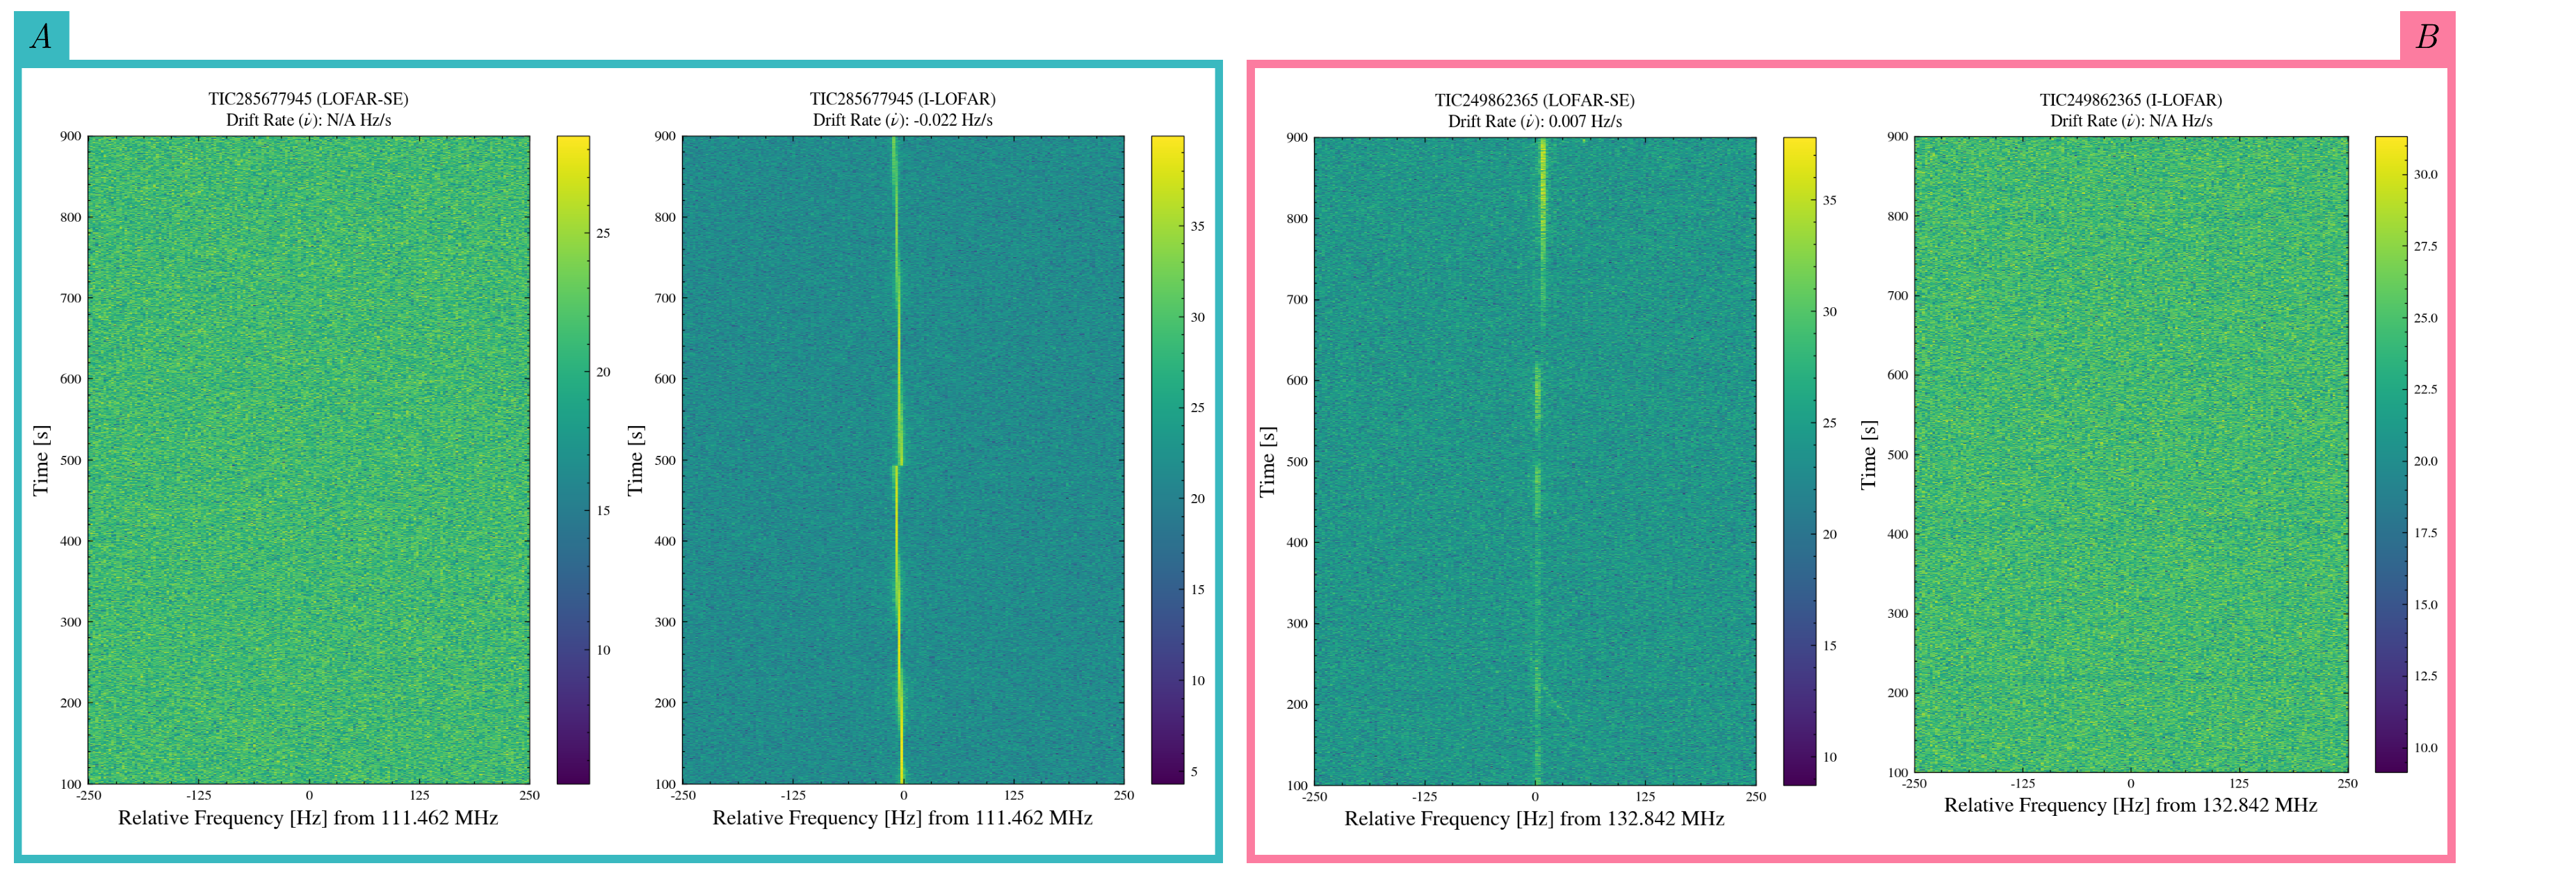
\includegraphics[width = \textwidth]{SETI/figures/narrowband/grid.png}
    \caption{Dynamic spectra (waterfall plots) of detected narrow-band signal centered on the detected frequency of detection, showing the two most common cases of coincidence rejection. Case A (\textit{left}) shows a narrowband signal with a non-zero drift rate detected at I-LOFAR and not LOFAR-SE. Case B \textit{(Right)} shows the opposite where a non-zero drift rate signal is not detected by I-LOFAR but is detected by LOFAR-SE. For a signal to be considered a detection of interest both sites would have to exhibit non-zero drift rate signal at the same frequency simultaneously. }
    \label{fig:coincidence_cases}
\end{figure}

 In the case of this study, a singular beam observes a single target for 15 minutes at both stations and observations are converted to barycentric reference frame. Narrow-band searches are then performed at both sites, and the results of both searches are compared. In \Cref{fig:coincidence_cases} two common detection cases are shown and how the use of dual site observation aids in the nature of each signals origin. 

\textit{Case A:} In this case a hit has been detected at the Irish station but is absent from the same frequency at the Swedish station. Thus the signal is rejected as a extraterrestrial emitter and deemed as RFI local to the Irish station. \\ 

\textit{Case B:} Similar to case A but this time the converse is seen, a hit has been detected at Swedish station and not at a the frequency at the Irish station. \\ 

In our analysis, a signal is classified as a mutual extraterrestrial hit only if two conditions are met: \textit{a)} the signals are within a frequency range of $\pm 4 \ \text{Hz}$ of each other in the barycentric reference frame, and \textit{b)} their drift rates are within $\pm 0.2 \ \text{Hz/s}$ of each other after barycentric drift corrections. In Figure \ref{fig:barycentric correction}, an intriguing candidate is depicted. In the topocentric frame, we detected a narrowband signal at 160 MHz that was simultaneously present at both stations. However, when converting to the barycentric reference frame (as illustrated in Figure \ref{fig:barycentric correction}), the signal appears to be seen at different frequencies with opposite signs due to the different line-of-sight velocities towards the target. As a result, this narrowband signal is rejected as a genuine sky-bound signal.

\begin{figure*}[]
    \centering
    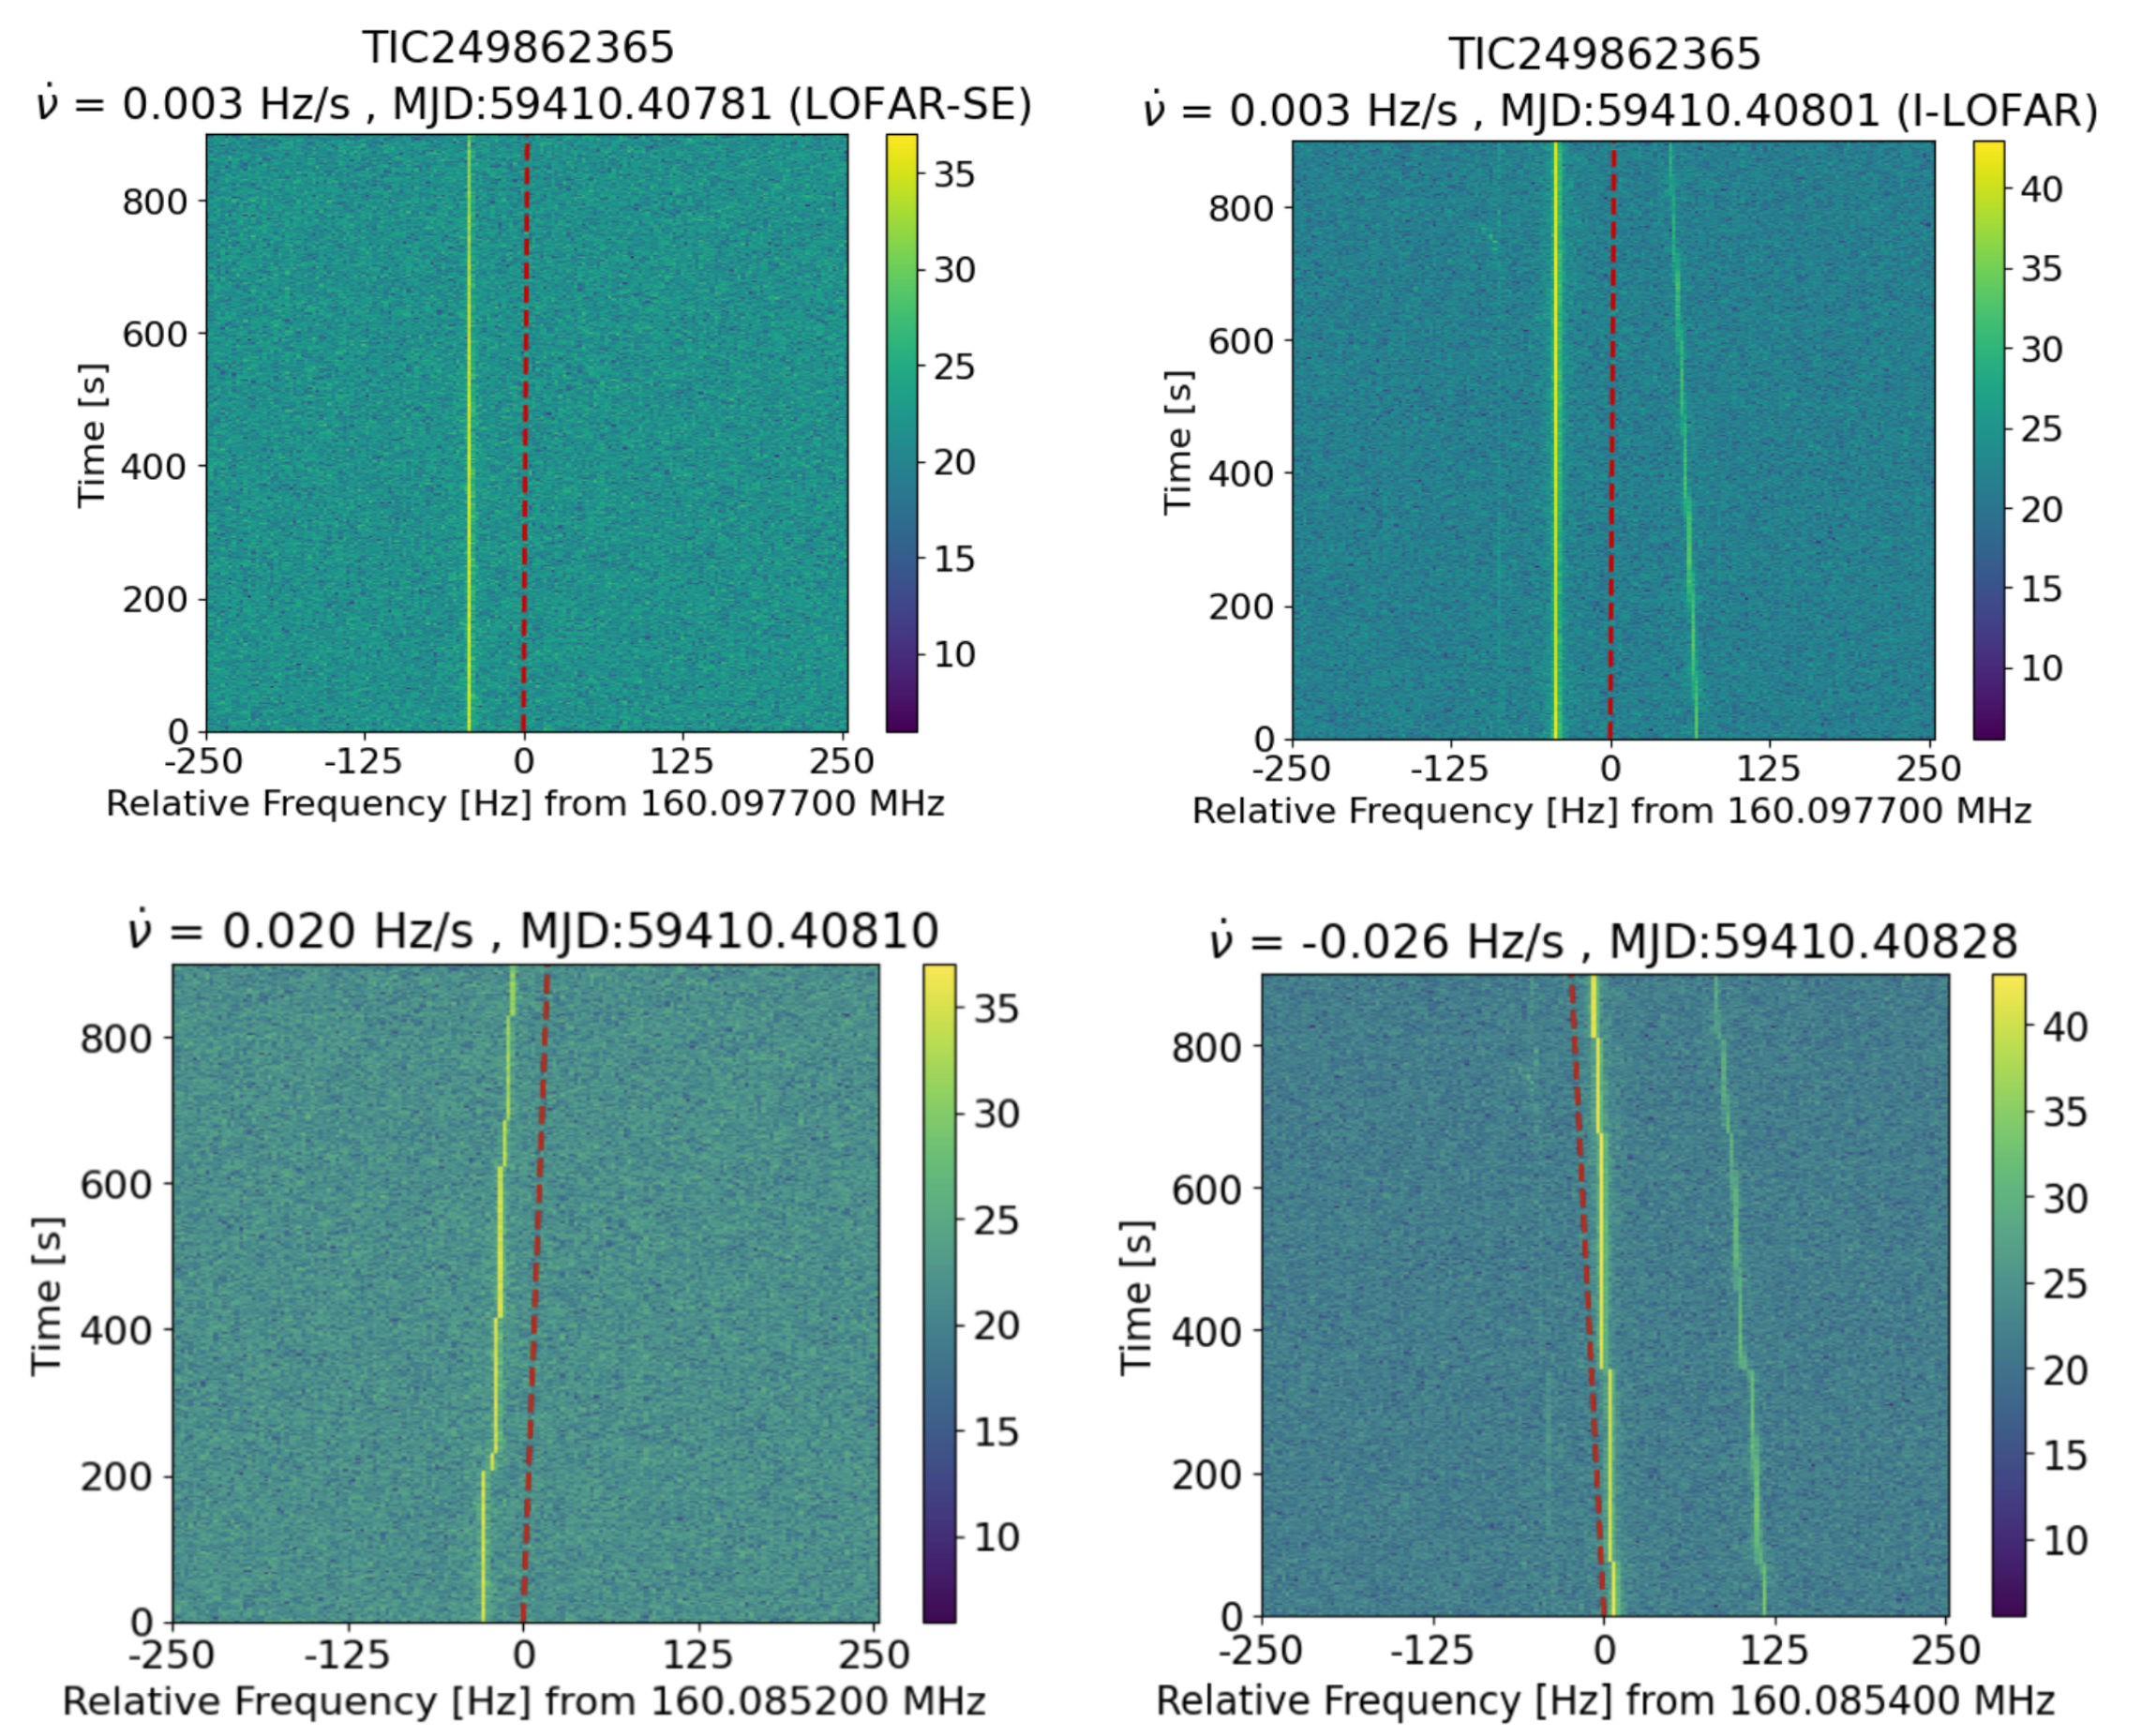
\includegraphics[width = 0.9\textwidth]{SETI/figures/narrowband/bary.correction.jpg}
  \caption{The \textit{top} two plots represent narrowband signals detected at both stations in the topocentric frame of reference. The \textit{bottom} two plots show the same detected narrowband signals detected at both stations but corrected to the barycentric frame of reference. This is illustrated by the newly added drift to signals present in the post correction.}
  \label{fig:barycentric correction}
\end{figure*}


\subsection{Search Results}

\Cref{fig:scatter_DR} depicts the observed drift rates as a function of frequency. As shown in \Cref{fig:histogram_hits_comparison}, a substantial number of hits are observed at 125 MHz and 138 MHz, suggesting the presence of potential aircraft communications within these frequency bands. Notably, at I-LOFAR, a significant number of hits are also detected at 167 MHz, which is suspected to be related to aircraft communication. Additionally, a pronounced spike in RFI at 164 MHz is observed at the Swedish station (LOFAR-SE), likely associated with marine communications due to the proximity of LOFAR-SE to the coast. \\ 

Implementing barycentric corrections and coincidence rejections, no signals of interest were identified among the observed candidates. Comprehensive information regarding the targets and their corresponding hits for both \textit{TESS} and \textit{Gaia} can be found in the supplementary databases presented in the Tables \ref{tab:TESS_results} and \ref{tab:Gaia_results}.


\begin{table}[ht]
  \centering
  \scriptsize % Shrink font size for wide table
  \caption{\textit{TESS} candidates used as bore sight pointings for the survey. These targets were selected from the NASA Exoplanet Archive (NEA) based on visibility at both LOFAR stations.}
  \label{tab:TESS_results}
  \begin{tabular}{
      S[table-format=9.0]   % TIC ID
      S[table-format=5.4]   % MBJD
      S[table-format=2.6]   % RA
      S[table-format=2.6]   % DEC
      S[table-format=4.2(3)] % Distance ±
      S[table-format=3.0]   % LOFAR-SE
      S[table-format=3.0]   % I-LOFAR
      S[table-format=1.0]   % Mutual
  }
  \toprule
  {\textbf{TIC ID}} & {\textbf{MBJD Start}} & {\textbf{RA (h)}} & {\textbf{DEC (°)}} & {\textbf{Dist. (pc)}} & {\textbf{LOFAR-SE}} & {\textbf{I-LOFAR}} & {\textbf{Mutual}} \\
  \midrule
  27677846  & 59410.3856 & 4.424676  & 46.365902 & 78.71(33)  & 294 & 151 & 0 \\
  51024887  & 59410.3189 & 2.810346  & 62.189260 & 41.53(16)  & 265 & 181 & 0 \\
  81831095  & 59410.3300 & 3.187109  & 61.762385 & 399.40(530) & 277 & 196 & 0 \\
  121966220 & 59410.3967 & 5.053188  & 41.785784 & 472.70(913) & 376 & 171 & 0 \\
  142090065 & 59402.4266 & 5.271567  & 79.737727 & 182.91(129) & 290 & 282 & 0 \\
  191146556 & 59410.4078 & 0.553625  & 46.340305 & 282.83(301) & 378 & 266 & 0 \\
  249862365 & 59410.3078 & 2.541534  & 52.704091 & 184.69(129) & 330 & 197 & 0 \\
  250724252 & 59410.2967 & 2.233683  & 53.121508 & \multicolumn{1}{c}{N/A} & 265 & 262 & 0 \\
  266500992 & 59410.3634 & 4.078149  & 52.256992 & 165.31(99)  & 276 & 164 & 0 \\
  288132261 & 59403.5613 & 13.965621 & 79.583322 & 154.94(52)  & 328 & 310 & 0 \\
  \bottomrule
  \end{tabular}
  
  \vspace{0.5em}
  \textit{Note:} First 10 entries shown. Full table available in the supplementary material. Distances are based on Gaia DR2 parallax and uncertainties are from \cite{TIC_Distances}. Asterisks denote confirmed NEA exoplanets.
  \end{table}  


  \begin{table}[ht]
    \centering
    \scriptsize % Reduce text size to fit wide table
    \caption{\textit{Gaia} candidates found within $1.295^\circ$ of \textit{TESS} boresight pointings. The \textit{Gaia} target pool is drawn from GDR3. Filtering was applied based on parallax error; targets with distance errors $>20\%$ were excluded to preserve EIRP sensitivity.}
    \label{tab:Gaia_results}
    \begin{tabular}{
        S[table-format=18.0]  % Gaia ID
        S[table-format=2.6]   % RA
        S[table-format=2.4]   % DEC
        S[table-format=4.3]   % Distance
        S[table-format=4.1]   % Teff
        S[table-format=1.3]   % Separation
        S[table-format=9.0]   % TIC ID
        S[table-format=3.0]   % LOFAR-SE
        S[table-format=3.0]   % I-LOFAR
        S[table-format=1.0]   % Mutual
    }
    \toprule
    {\textbf{\textit{Gaia} ID}} & {\textbf{RA (°)}} & {\textbf{DEC (°)}} & {\textbf{Dist. (pc)}} & {$T_{\text{eff}}$ (K)} & {\textbf{Separation (°)}} & {\textbf{TIC ID}} & {\textbf{LOFAR-SE}} & {\textbf{I-LOFAR}} & {\textbf{Mutual}} \\
    \midrule
    540394404387737000 & 0.003867 & 77.7984 & 850.636 & 4954.0 & 1.129 & 407394748 & 257 & 181 & 0 \\
    540420788369495000 & 0.008171 & 77.9843 & 836.863 & 5387.3 & 1.093 & 407394748 & 257 & 181 & 0 \\
    540290637978301000 & 0.011819 & 77.5007 & 563.690 & 4686.4 & 1.013 & 407394748 & 257 & 181 & 0 \\
    540431753423271000 & 0.017921 & 78.2404 & 1293.320 & 5365.0 & 1.295 & 407394748 & 257 & 181 & 0 \\
    540422957330267000 & 0.018887 & 78.0603 & 722.054 & 5415.4 & 0.958 & 407394748 & 257 & 181 & 0 \\
    564460068219877000 & 0.018908 & 78.4901 & 1415.490 & 5276.0 & 1.189 & 407394748 & 257 & 181 & 0 \\
    540394400090438000 & 0.020346 & 77.7933 & 861.226 & 5896.3 & 1.118 & 407394748 & 257 & 181 & 0 \\
    540387257562774000 & 0.021907 & 77.6559 & 818.213 & 4952.0 & 0.947 & 407394748 & 257 & 181 & 0 \\
    564451272126871000 & 0.022257 & 78.3080 & 854.196 & 4731.2 & 1.089 & 407394748 & 257 & 181 & 0 \\
    540291153374376000 & 0.022550 & 77.5313 & 1105.790 & 4892.0 & 0.985 & 407394748 & 257 & 181 & 0 \\
    \bottomrule
    \end{tabular}
    
    \vspace{0.5em}
    \textit{Note:} First 10 entries shown. Full table is available in the paper's supplementary material. The table includes each \textit{Gaia} target near a \textit{TESS} pointing and its angular separation from the LOFAR beam boresight.
    \end{table}
    